\documentclass[border=10pt]{standalone}
\usepackage{pgfplots}
\pgfplotsset{compat=1.18}
\begin{document}
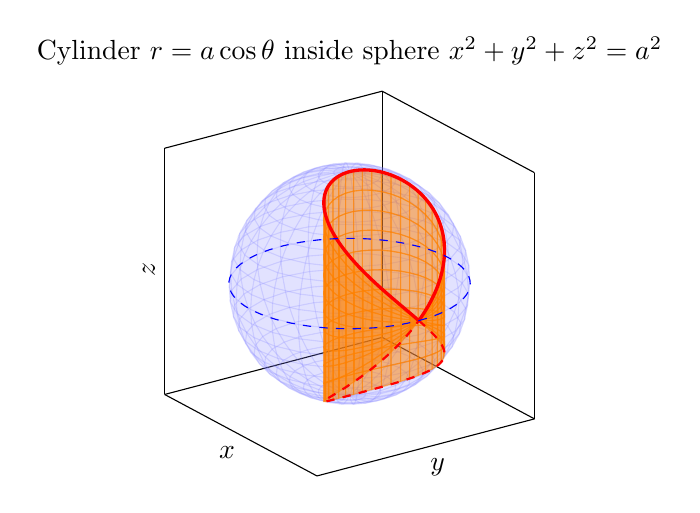
\begin{tikzpicture}
\begin{axis}[
    view={55}{22},
    axis equal image,
    xlabel={$x$}, ylabel={$y$}, zlabel={$z$},
    xmin=-1.1, xmax=1.1, ymin=-1.1, ymax=1.1, zmin=-1.1, zmax=1.1,
    ticks=none,
    title={Cylinder $r=a\cos\theta$ inside sphere $x^2+y^2+z^2=a^2$}]
% sphere (semi-transparent)
\addplot3[surf, shader=flat, opacity=0.12, color=blue!50,
    domain=0:360, samples=25, y domain=0:180, samples y=25,
    z buffer=sort]
    ({cos(x)*sin(y)}, {sin(x)*sin(y)}, {cos(y)});
% cylinder clipped to sphere: zmax = abs(sin(t/2))
\addplot3[surf, shader=flat, opacity=0.5, color=orange,
    domain=0:360, samples=40, y domain=-1:1, samples y=12,
    z buffer=sort]
    ({0.5+0.5*cos(x)}, {0.5*sin(x)}, {y*abs(sin(x/2))});
% top rim: cylinder meets sphere
\addplot3[red, very thick, domain=0:360, samples=100, samples y=0]
    ({0.5+0.5*cos(x)}, {0.5*sin(x)}, {abs(sin(x/2))});
% bottom rim
\addplot3[red, dashed, thick, domain=0:360, samples=100, samples y=0]
    ({0.5+0.5*cos(x)}, {0.5*sin(x)}, {-abs(sin(x/2))});
% equator
\addplot3[blue, dashed, domain=0:360, samples=80, samples y=0]
    ({cos(x)}, {sin(x)}, {0});
\end{axis}
\end{tikzpicture}
\end{document}